\documentclass{article}

\usepackage{authblk}
\usepackage{amsmath}
\usepackage{tikz}
\usepackage{chngcntr}
\usepackage{caption}
\usepackage{subcaption}
\usepackage{lipsum}

\usepackage{titlesec}

\makeatletter
\newcommand{\setappendix}{Appendix~\thesection:~}
\newcommand{\setsection}{\thesection~}
\titleformat{\section}{\bfseries\LARGE}{%
  \ifnum\pdfstrcmp{\@currenvir}{appendices}=0
    \setappendix
  \else
    \setsection
  \fi}{0em}{}
\makeatother

\usepackage[titletoc]{appendix}

\counterwithin{figure}{section}

\author{Aurora Zuoris \\ \normalsize{aurora.zuoris101@alu.ulpgc.es}}
\affil{Universidad de Las Palmas de Gran Canaria}
\title{Matrix multiplication at the speed of light}

\begin{document}

\maketitle

\abstract{
This paper will discuss various methods for implementing matrix multiplication,
along with their advantages and disadvantages for different situations.
Languages explored are Python, Java, C, Rust, and SQL, with methods including
naive, improving cache hits, parallelization, vectoring and trying to leverage the GPU.
}

\section{Introduction}

Matrix multiplication is becoming increasingly important in the modern world.
Two big examples are machine learning and graph theory, both of which are
becoming more and more important with the rise of big data.
Thus knowing what the best ways to implement matrix multiplication in
various situations is crucial for the future of computing.

In this paper, we will explore various ways to speed up matrix multiplication.
One major use for matrix multiplication in the past decade is in deep machine learning,
as they are used to represent the weights and biases of neural networks, such that
a forward pass can be done by multiplying the input by the weight matrix and adding the bias vector,
limiting the speed of the forward pass to the speed of matrix multiplication.

\section{Methotology}

The matrix multiplication algorithms will be implemented in various languages, using a plethora
of different optimization techniques, and then benchmarked to see which is the fastest using each
language's timing libraries to get the most accurate results possible.

For brevity and because of time constraints, not all possible combinations of languages and optimization
techniques will be explored, but rather a subset of the most interesting ones.

\subsection{Python}

To start with, python will be used as a baseline, as it is commonly used in machine learning and it's known to be slow.
So it will be interesting to see how much of a difference there is between python and other languages.

The python implementation consists of a class with a field for the matrix, and a method for multiplying two matrices.
The multiplication is implemented using list comprehension, which is more pythonic than using for loops, and can be faster too
given that they use more optimized code under the hood. Making it a more fair comparison to other languages.

The code used is as follows:

\subsection{Java}

Java is a language that is commonly used in industry, and it's known to be faster than python.
The implementation is similar to the python one, with a class for the matrix and a method for multiplying two matrices.
The multiplication is implemented using for loops, as they are the most common way to do it in java.
For the matrix itself, it is implemented with a 1D array, storing the matrix in row-major order.
This is done as it's unnecessary to do $N+1$ allocations for a matrix of size $N\times N$,
when it can be done with just one allocation. Aditionally, being explicit about the order of the matrix in memory
is a good way to improve cache hits, as will be seen later, and also leads to better self documentation.

The implementation is as follows:

\subsection{C}

For C, we will first do a naive implementation, and then we will try to improve it.
The naive implementation is similar to the java one, an allocation in row-major order, and then a function that simply does a nested for loop.
It is also worth noting that in C, it'll also be important what optimization flags are used when compiling, as they can make a big difference.

The implementation is as follows:

\newpage

\subsection{C with cache locality}

The first improvement we will try to do is to improve cache hits.

One way to improve the speed of matrix multiplication is to try to improve cache hits.
This can be done by having the second matrix be looped by rows in the inner loop.
While this does not correspond to an actual matrix multiplication, as the second matrix is looped trough incorrectly, it does
correspond to $AB^\top$. To fix this discrepancy, one needs to first do a transpose on the second vector.
While this is extra computation that needs to be done, a transposition is $O(n^2)$ in time complexity, while the multiplication
is $O(n^3)$, so while it may seem like it would slow it down, you can think of this addition as procuring $O(n^2)$ work to have
$O(n^3)$ computations be up to $200$ times faster, or however much faster it is to fetch data from the cache rather than the RAM.
This can be visualized in figure \ref{fig:cache}.


\begin{figure}[h!]
	\begin{subfigure}{0.3\textwidth}
		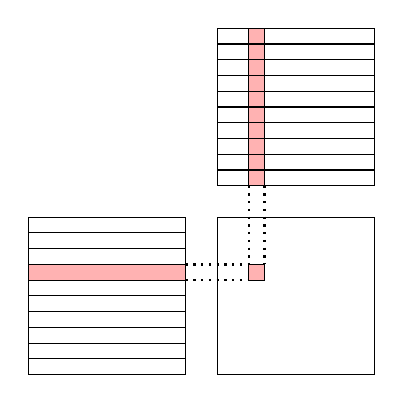
\begin{tikzpicture}[scale=0.2]
			\draw (0,0) rectangle +(10,10);
			\foreach \y in {1, ..., 9}
			{
				\draw (0, \y) -- (10, \y);
			}
			\filldraw[fill=red!30!white] (0, 6) rectangle +(10, 1);
			\draw (12,0) rectangle +(10, 10);
			\draw (12, 12) rectangle +(10, 10);
			\filldraw[fill=red!30!white] (14, 12) rectangle +(1, 10);
			\foreach \y in {1, ..., 9}
			{
				\draw (12, 12+\y) -- +(10, 0);
			}
			\draw[dotted, thick]
				(10, 6) -- (14, 6)
				(10, 7) -- (14, 7)
				(14, 12) -- (14, 7)
				(15, 12) -- (15, 7)
				;
			\draw[fill=red!30!white] (14, 6) rectangle +(1, 1);
		\end{tikzpicture}
	\caption{
		naive multiplication has a lot of cache misses
	}
	\end{subfigure}
	\hfill
	\begin{subfigure}{0.3\textwidth}
		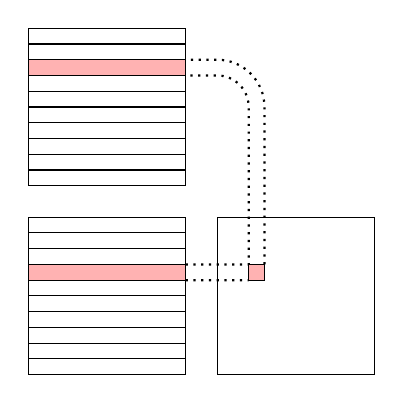
\begin{tikzpicture}[scale=0.2]
			\draw (0,0) rectangle +(10,10);
			\filldraw[fill=red!30!white] (0, 6) rectangle +(10, 1);
			\foreach \y in {1, ..., 9}
			{
				\draw (0, \y) -- (10, \y);
			}
			\draw (12,0) rectangle +(10, 10);
			\draw (0, 12) rectangle +(10, 10);
			\filldraw[fill=red!30!white] (0, 12+7) rectangle +(10, 1);
			\foreach \y in {1, ..., 9}
			{
				\draw (0, 12+\y) -- +(10, 0);
			}
			\draw[dotted, thick]
				(10, 6) -- (14, 6)
				(10, 7) -- (14, 7) -- (14, 17) arc[start angle=0, end angle=90, radius=2] -- (10, 12+7)
				(15, 7) -- (15, 17) arc[start angle=0, end angle=90, radius=3] -- (10, 12+8)
				;
			\draw[fill=red!30!white] (14, 6) rectangle +(1, 1);
		\end{tikzpicture}
	\caption{
		$AB^\top$ has more cache hits
	}
	\end{subfigure}
	\caption{Matrix multiplication cache hit optimization}
	\label{fig:cache}
\end{figure}

\subsection{C with parallelization}

Finally for C, the most optimized version will be implemented, attempting to use both parallelization and vectorization.
This implementation uses pthreads to parallelize the multiplication, and SIMD intrinsics to vectorize it.
This is done by splitting the elements of the matrix into chunks, and then having each thread calculate the result for all the elements in its chunk.
As the chunks are independent, and the two input matrices are only ever read, this is a safe operation to do in parallel without any need for synchronization other than joining
the threads at the end.

\subsection{Rust with GPU}

Last but not least, we will try to leverage the GPU to speed up matrix multiplication.
For this, we will use the rust programming language, as it has a good, modern library for GPU programming called wgpu.

WGPU is based on the WebGPU standard, which is a new upcoming standard for GPU programming meant to target the web and replace WebGL.
It may seem strange to use a web standard for GPU programming, but it is actually a good idea, as modern web standards are designed to be
highly portable and as fast as native applications, meaning that using modern web standards will lead to programs that are as fast as native ones,
and can be run on any platform, from desktops to mobile phones, to even web browsers.
It is notable to say that even if it is a web standard, one can still use it to make native applications, as it is not tied to the web in any way
other than its origins.

This leads to a very portable and fast library that can leverage the GPU, unlike most other libraries that use the GPU which
are usually tied to a specific platform, such as CUDA, which is only available on Nvidia GPUs and only on desktops, which also need meticulous setup
to get working correctly. WebGPU on the other hand, compiles to SPIR-V, which is a standard intermediate representation for shaders, which can then be
compiled to native code for any platform, and can be run on any platform that supports Vulkan, DirectX 12, Metal, or OpenGL, which is almost all of them.
Leading to a very simple, batteries included library that can be used to leverage the GPU for any platform.

A notable trivia about the specific library used here, wgpu, is that it's one of the two main implementations of WebGPU, being used in the Firefox browser to implement WebGPU.
The other implementation being Dawn, written in C++, which is used in Chromium browsers to implement WebGPU.

Unlike other implementations, this one is much more convoluted, as it is not as simple as just calling a function to do matrix multiplication,
but rather it needs to be done in a shader, which is a program that runs on the GPU, and is written in a special language called WGSL.
And thus there also is lots of boilerplate code to set up the GPU, and to pass the matrices to the shader, and to get the result back.
To get a full explanation of how this works, see appendix \ref{sec:wgpu}.
This also has implications when it comes to benchmarking, as one could either just measure the time it takes to do the computations on the GPU,
or also include the time it takes to move the data to and from the GPU, which is a much more expensive operation than the actual computation.

\section{Results}

\section{Conclusion}

\section{Future Work}

\begin{appendices}

\appendix

\section{Implementing matrix multiplication in Wgpu}

 \label{sec:wgpu}


\end{appendices}


\end{document}